\section{Fundamentals of \ac{SSO}}

% Maybe section about authentication and authorization
\subsection{Basics of Authentication}
\subsubsection{Authentication \& Authorization}

Authentication is the act of establishing a users identity. The user has to prove, that he is who he says
he is\footcite[Cp.][p. 398]{Basavala2012}.
There are three main ways how a user can prove his identity:
\begin{enumerate}
    \item The user provides some secret, that only he knows, e.g. a password.
    \item The user provides something, that only he has.
          An example for this is an \ac{SMS} based authentication system, where the user receives a message with a code,
          which has to be entered into the login form. He thus proves, that he is in possession of the phone with the phone
          number he has previously provided.
    \item The user proves his identity by using some unique physical characteristic, e.g. a fingerprint or eye retina scan.\footcite[Cp.][p. 398]{Basavala2012}
\end{enumerate}
Using only one of these ways to authenticate a user is called \ac{SFA}, using two is called \ac{2FA} and using 
multiple factors is called \ac{MFA}.
Using two or more factors for authentication improves security and is deemed essential for applications with sensitive data.\footcite[Cp.][]{Drew2019}

Contrary to authentication, authorization determines, wether a user is allowed to access a specific resource.
It happens once the user has been authenticated.\footcite[Cp.][]{Auth0AuthNvsAuthZ} For example, user A might make a post on a social media site,
which is only shared with his close friends. If another user B wants to view the post, the system first checks
if user B is part of user A's close friends. If he is, he is authorized to see the resource.

\subsubsection{Authentication flows without SSO}

Figure \ref{fig:sfa_flow_chart} shows a flow chart for a traditional authentication flow using a username and password.
The user enters his information and clicks the "Sign In" button. Next, the server checks in the database,
wether or not the username exists and the password is correct. If this is true, the user is authenticated
and he can enter the website.\footcite[Cp.][p. 400]{Basavala2012}

\begin{figure}[H]
    \centering
    \caption{Flow chart of SFA authentication process}
	\label{fig:sfa_flow_chart}
    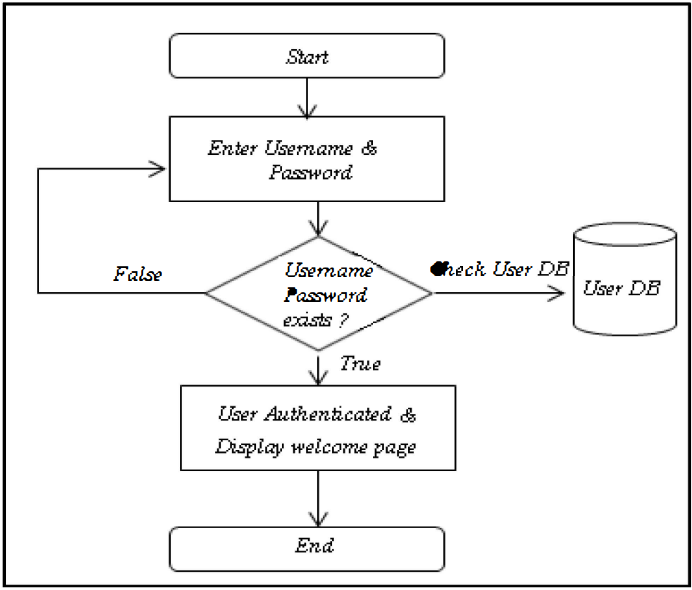
\includegraphics[width=0.5\textwidth]{sfa_flow_chart.png}
    \\
    \cite[Source:][]{Basavala2012}
\end{figure}

Using \ac{2FA} introduces complexity into this process, as the user now has to additionally provide something he has.
In the case of \ac{SMS} \ac{2FA} there are now multiple databases needed to store passwords,
phone numbers and the codes sent via \ac{SMS}\footcite[Cp.][p. 400]{Basavala2012}. 
Additionally, software needs to be operated which generates the
codes and sends them to the user.
Managing this complexity and ensuring security for all components is both time- and cost-intensive.

\subsection{Single Sign-On and Federated Identity}
\subsubsection{Definitions}

\textbf{\ac{SSO}} is a mechanism which allows users to sign into multiple independent software systems
using a single set of credentials\footcite[Cp.][134]{Radha2012}.
It also only requires the user to perform a single action to authenticate against multiple participating services.
Such systems or services could be apps, websites or technical interfaces like \acp{API}.
After signing in, the user is not asked to enter their password again when visiting a different service\footcite[Cp.][p. 18]{Bazaz2016}

\ac{SSO} is made possible by an \textbf{\ac{IdP}}, which provides a central server for authentication.
When talking about \ac{SSO}, the website operator is usually refered to as \textbf{\ac{SP}}.
The users authenticate with the \ac{IdP} and it shares the user's identity with the \ac{SP}.\footcite[Cp.][p. 24]{Beltran2016}
The \ac{SP} does not confirm the user's identity in any way, so he has to trust the \ac{IdP} to correctly
deliver user identities\footcite[Cp.][]{Nallathamby2018}.
Originally, \ac{SSO} could only be used by members of a single organization to sign into different 
applications like HR software, payroll or communication systems, because there were no open standards,
that allowed companies to share identities with other organizations.\footcite[Cp.][]{OktaFIM}

\ac{FIM} is the broader term for managing user identities across apps and websites from different companies.
It provides standards which companies can use to share user identities between trusted domains,
which allows \ac{SSO} to be deployed not just in organizations, but also on the open web.
These standards are what allows end-users to use \acp{IdP} like Google and Facebook to sign into many
different websites.\footcite[Cp.][]{OktaFIM}

\subsubsection{Types \& Use-Cases of SSO}

Figure \ref{fig:sso_types} shows the different types of \ac{SSO}.
Intranet \ac{SSO} is used within the secure network of an organization and allows its members to 
access multiple applications with one set of credentials. This is relatively easy to deploy, as all components
and clients are administrated by the same organization, eliminating the need for open standards and trust to
third parties.
Extranet \ac{SSO} connects applications and \acp{SP} from different organizations.
This is the basis for Web \ac{SSO}, which is the type this paper is concerned with.
It is based on web technologies and allows users to access different websites with a single set of credentials.\footcite[Cp.][p. 135]{Radha2012}

\begin{figure}[H]
    \centering
    \caption{Types of Single Sign-On}
	\label{fig:sso_types}
    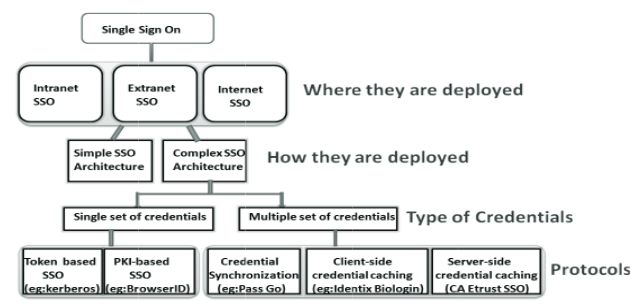
\includegraphics[width=0.8\textwidth]{sso_types.png}
    \\
    \cite[Source:][]{Radha2012}
\end{figure}

\subsubsection{Web SSO Protocols \& Technologies}

There are many different protocols defined for \ac{SSO}.
Some are only used for Intranet \ac{SSO}, which is not covered in this paper.
The next section will therefore only cover the three most used Web \ac{SSO} protocols\footcite[Cp.][]{OneLoginFIMTechnologies}.

\textbf{Security Assertion Markup Language}

\ac{SAML} is an open standard for exchanging user identities and authorization information between
an \ac{IdP} and a service provider.
It uses the markup language XML for communication between applications.
The typical authentication flow using \ac{SAML} is shown in figure \ref{fig:flow_saml}.
An \ac{SP} contacts an \ac{IdP} and requests a user identity.
The \ac{SAML} standard does not specify how the \ac{IdP} has to authenticate the user,
but only defines the communication between the two parties.
After the user has authenticated with the \ac{IdP} the identity information is sent back to 
the \ac{SP}. It includes, whether the user is authenticated, what roles and rights they have and
which data and resources they are allowed to access.\footcite[Cp.][p. 137]{Radha2012}
Note that while the \ac{SP} basically communicates directly with the \ac{IdP}, all communication
still goes through the user. Which \ac{IdP} is used is predefined by the \ac{SP}, the user does not
get to choose where they enter their credentials or who provides their identity.
The \ac{SP} has to trust the \ac{IdP} completely, because it also provides authorization information.

\begin{figure}[H]
    \centering
    \caption{Flow of SAML Protocol}
	\label{fig:flow_saml}
    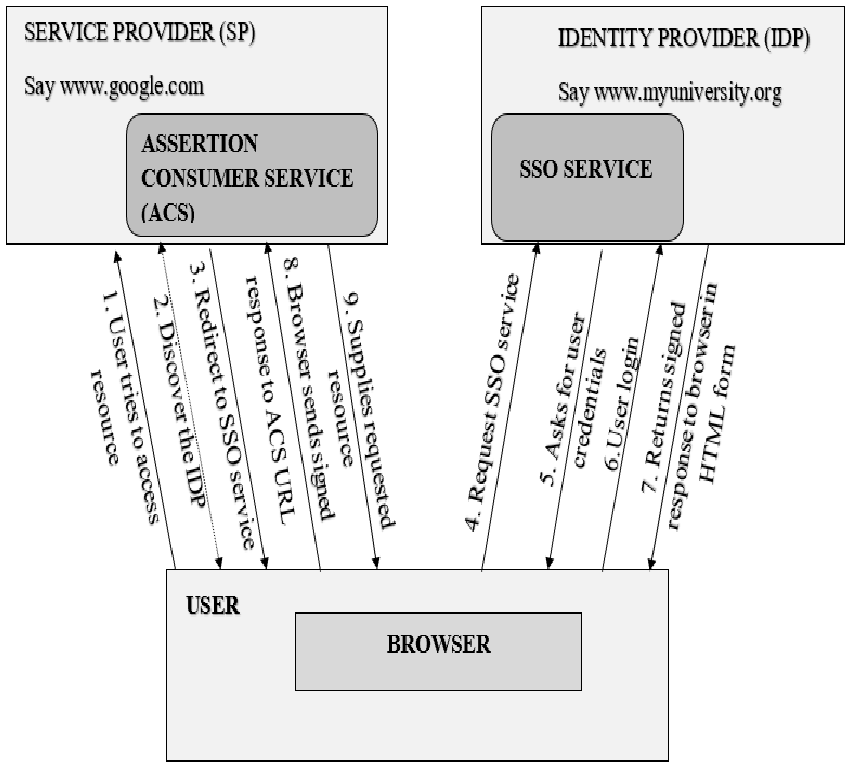
\includegraphics[width=0.5\textwidth]{flow_saml.png}
    \\
    \cite[Source:][p. 21]{Bazaz2016}
\end{figure}

\textbf{OpenID}

This protocol works differently than \ac{SAML}, in that the user gets to choose who provides their identity.
They might use a large \ac{IdP} like Google or Facebook or even set up their own OpenID service.
The \ac{SP} is called the \ac{RP} in this model. The \ac{IdP} is only responsible for authentication of users
and providing identity. It does not deliver any other authorization information.\footcite[Cp.][p. 21]{Bazaz2016}
The flow is shown in figure \ref{fig:flow_openid} and works like this.
The user visits the website and clicks the sign in button. They are then prompted to enter their OpenID identity provider.
The \ac{RP} (so the website) then redirects the user to the site of the \ac{IdP}, where the user authenticates by
entering their credentials. In the next step the user tells the \ac{IdP}, which information they want to share with
the \ac{RP}. If the credentials are valid, the selected identity information is passed to the \ac{RP}, otherwise
the user is asked to enter valid credentials.\footcite[Cp.][p. 21]{Bazaz2016}
This seperation of \ac{RP} and \ac{IdP} and introduction of user choice is the basis for Web \ac{SSO} as we know it,
where websites allow users to choose their preferred identity provider.
\ac{SAML} does not allow for this, as the \ac{IdP} is predefined by the \ac{SP}.

\begin{figure}[H]
    \centering
    \caption{Flow of OpenID Protocol}
	\label{fig:flow_openid}
    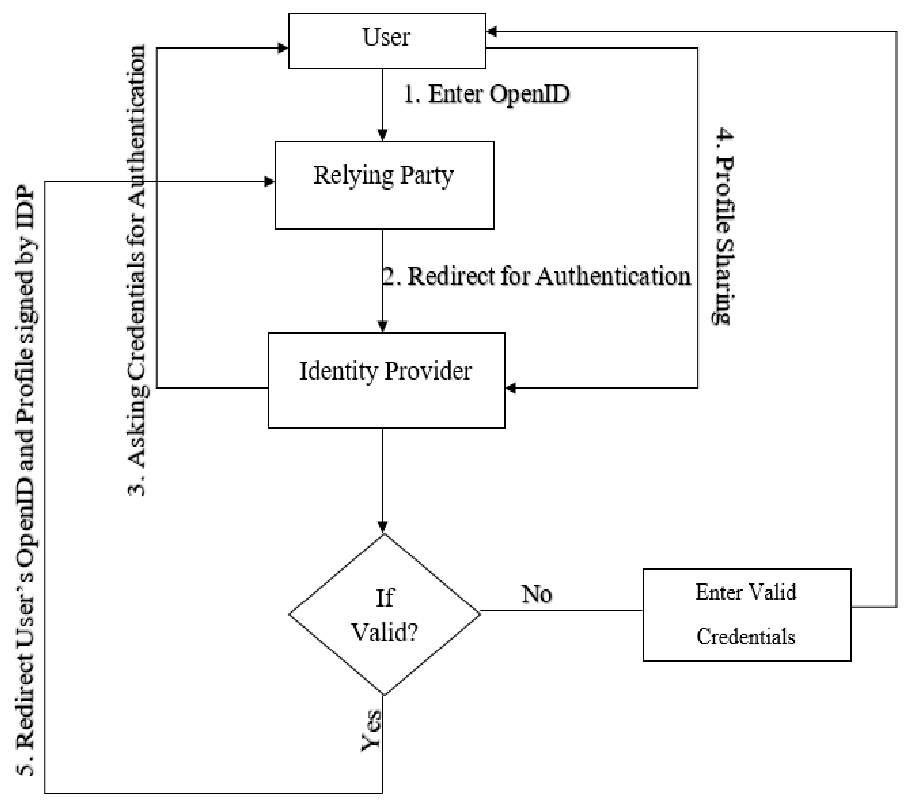
\includegraphics[width=0.5\textwidth]{flow_openid.png}
    \\
    \cite[Source:][p. 22]{Bazaz2016}
\end{figure}

\textbf{OAuth 2.0 \& OpenID Connect}

This \ac{SSO} protocol differentiates from the others, in that it centers around authorization rather than authentication.
An example use-case for this is a third-party app wanting to create a Facebook post in the user's name on their profile.
For this, the app does not need an identity, but rather the permission from Facebook to create a post.
It contacts Facebook's OAuth Server and asks it for permission. Facebook then contacts the user which owns the resource
(in this case the Facebook account) and asks them for permission. They accept by logging into their account and accepting
access from the app. The Facebook OAuth Server sends back a token to the app which can be used to create the post.
The app then contacts Facebook's Resource Server to actually create the post, providing the token to prove it is authorized.\footcite[Cp.][]{Wesener2021}

\begin{figure}[H]
    \centering
    \caption{Flow of OAuth 2.0 Protocol}
	\label{fig:flow_oauth2}
    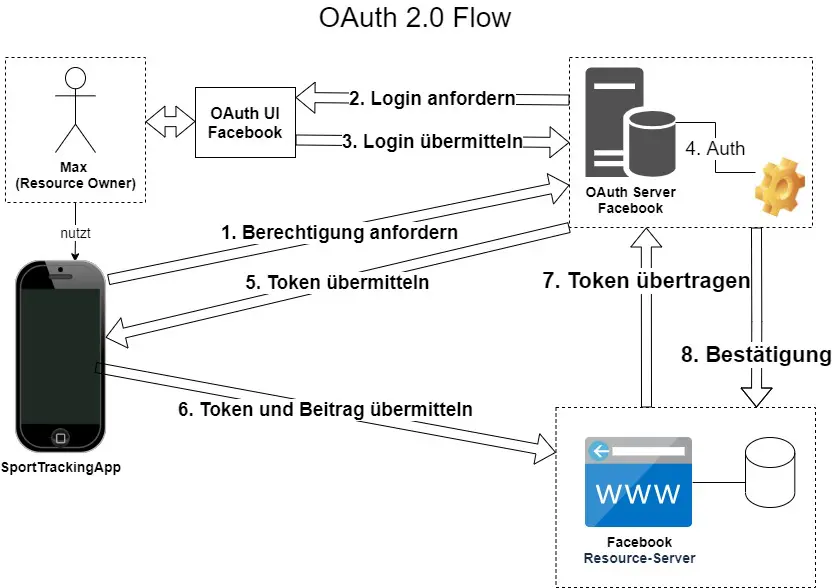
\includegraphics[width=0.8\textwidth]{flow_oauth2.png}
    \\
    \cite[Source:][p. 22]{Wesener2021}
\end{figure}

While OAuth 2.0 is a protocol specification, OpenID Connect is a concrete implementation of the protocol.
The terms "OpenID" and "OpenID Connect" are different and can't be used interchangably.\footcite[Cp.][]{Wesener2021}

To further understand the difference between the OAuth 2.0 und OpenID functionalities consider an e-commerce example,
where the user has to enter their payment information. They have previously entered it into their Google account and would
like to automatically fill the information from Google into the shop.

Using OpenID, the shop would use Google as an \ac{IdP} to get the user's identity and automatically create a corresponding
user account on the website. As OpenID simply provides the identity and can't provide the payment information from Google,
the user would still have to enter their payment information manually.
It would then be saved in the user's account on the web shop (not Google) and when he returns to buy a different item,
the information could be retrieved from the \ac{SP}'s server.

With OAuth, the \ac{SP} would not have to create a user account using the identity from Google and would not have to store any
information on its server. It would simply request access to the payment information resource from Google. The user would
authenticate and allow the information transfer. Then the \ac{SP} could retrieve the information from Google and use it
in the checkout process.

\subsection{Web SSO Providers}

\subsubsection{Overview}

There are many \ac{SSO} solutions targeted at businesses for internal use.
In addition to an \ac{IdP} service they often provide an identity management suite which allows businesses
to easily deploy \ac{SSO} within their network.
The solutions targeting end users on the open web are often called "Social Login" services, as they rely on 
social networks that have a wide userbase like Facebook, Twitter, Google or LinkedIn.

The most popular social networks worldwide are Facebook with 2.9 billion and YouTube with 2.6 billion monthly 
active users\footcite[Cp.][]{StatistaSocial2022}.
As YouTube is based on user accounts from Google, the social login offerings of Google and Facebook are examined.

\subsubsection{Sign In With Google}
\label{sec:sign_in_with_google}

Google's service is based on the OAuth 2.0 protocol. This ensures a flexible service,
as \acp{SP} can create a seperate account on their server but do not have to, as they can retrieve
required resources using OAuth.\footcite[Cp.][]{GoogleSignIn2022}
Customizable buttons are provided by Google which redirect the user to Googles sign in page (figure \ref{fig:google_sign_in_ui}a).
Google claims data from the feature is not used for advertising or other non-related purposes.
If users are already signed into their Google account when visiting the website, Google offers the
possibility to sign in with one click using a pop up, as shown in figure (figure \ref{fig:google_sign_in_ui}b).
Google offers an additional autorization interface to allow loading other data from a users Google account.\footcite[Cp.][]{GoogleSignIn2022}

\begin{figure}[H]
    \caption{Sign In With Google UI}%
    \centering
    \subfloat[Sign In With Google Button]{{
\includegraphics[width=0.2\textwidth]{google_sign_in_button.png}}}%
    \hfill
    \subfloat[One-Tap Sign In]{{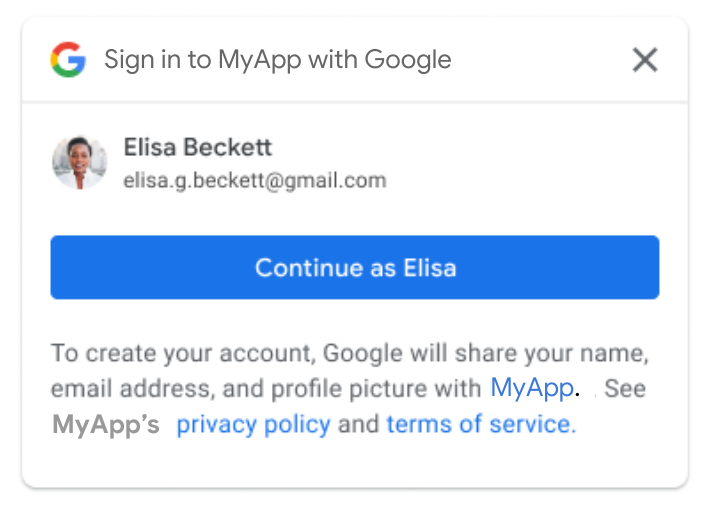
\includegraphics[width=0.3\textwidth]{google_one_tap.png}}}%
    \hfill
    \subfloat[Google Password Prompt]{{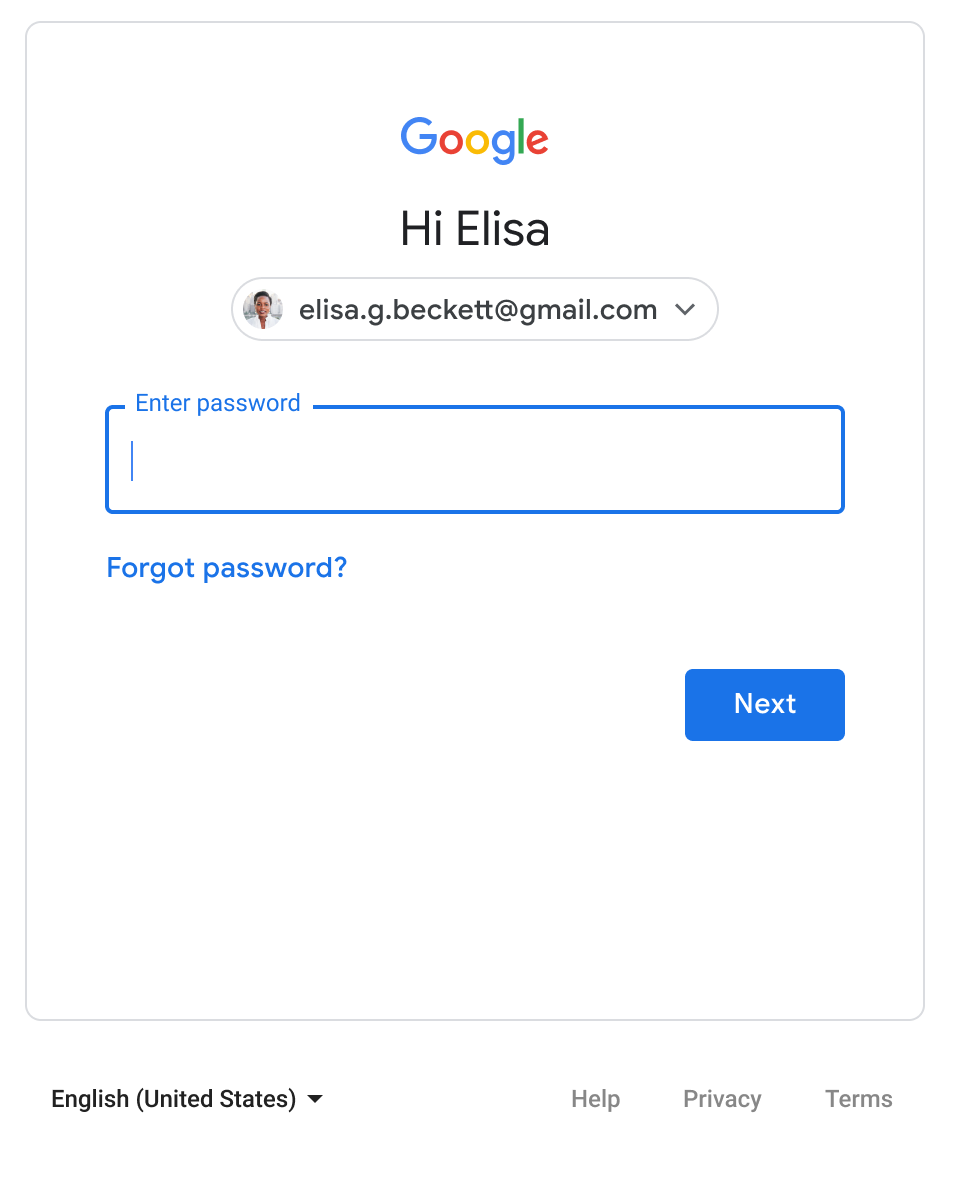
\includegraphics[width=0.4\textwidth]{google_password_prompt.png}}}%
    \cite[Source:][]{GoogleSignIn2022}
    \label{fig:google_sign_in_ui}%
\end{figure}

Integrating the Sign In With Google service into an existing website is fairly easy.
\acp{SP} have to create a project on Google's developer website. They then have the option
to configure the consent screen shown to the user by Google and enter e.g. their website name and logo,
a support e-mail adress and which user data the application wants to retrieve.\footcite[Cp.][]{GoogleSignIn2022}

Website developers can integrate Google's authentication interface into the website with just a few lines of code.
After the user authenticates, the user data is delivered into the web application and can be used from there.
If \acp{SP} have existing account management infrastructure, integrating this method might certainly require
more time, as data might come in a different format or database structures might not line up.\footcite[Cp.][]{GoogleSignIn2022}






%https://developers.google.com/identity/gsi/web/guides/overview

%\subsection{Security Considerations}
%
%When handling authentication on the website, the service provider (owner of the website) is solely responsible for ensuring security to prevent data breaches and leaked passwords.
%Research is constantly being conducted in the field of password and database security and there are multiple
%standards, which should be adhered to in order to maximize security.
%The United States \ac{NIST} publishes a set of digital identity guidelines, which outlines best practices
%for website developers.
%When designing a sign in form, developers have to specify certain requirements for user passwords.
%For example, a password should have a certain length and complexity

% https://auth0.com/blog/dont-pass-on-the-new-nist-password-guidelines/
%
%

%\subsection{Integration into existing websites}

%\subsection{User Tracking with \ac{SSO}}